% Template for PLoS
% Version 1.0 January 2009
%
% To compile to pdf, run:
% latex plos.template
% bibtex plos.template
% latex plos.template
% latex plos.template
% dvipdf plos.template

\documentclass[10pt]{article}\usepackage{graphicx, color}
%% maxwidth is the original width if it is less than linewidth
%% otherwise use linewidth (to make sure the graphics do not exceed the margin)
\makeatletter
\def\maxwidth{ %
  \ifdim\Gin@nat@width>\linewidth
    \linewidth
  \else
    \Gin@nat@width
  \fi
}
\makeatother

\IfFileExists{upquote.sty}{\usepackage{upquote}}{}
%%% NEED TO RM BOX SHADING AND TEXT-HIGHLIGHTING FOR PLoS ONE standards
\definecolor{fgcolor}{rgb}{0,0,0}
\newcommand{\hlnumber}[1]{\textcolor[rgb]{0,0,0}{#1}}%
\newcommand{\hlfunctioncall}[1]{\textcolor[rgb]{0,0,0}{\textbf{#1}}}%
\newcommand{\hlstring}[1]{\textcolor[rgb]{0,0,0}{#1}}%
\newcommand{\hlkeyword}[1]{\textcolor[rgb]{0,0,0}{\textbf{#1}}}%
\newcommand{\hlargument}[1]{\textcolor[rgb]{0,0,0}{#1}}%
\newcommand{\hlcomment}[1]{\textcolor[rgb]{0,0,0}{#1}}%
\newcommand{\hlroxygencomment}[1]{\textcolor[rgb]{0,0,0}{#1}}%
\newcommand{\hlformalargs}[1]{\textcolor[rgb]{0,0,0}{#1}}%
\newcommand{\hleqformalargs}[1]{\textcolor[rgb]{0,0,0}{#1}}%
\newcommand{\hlassignement}[1]{\textcolor[rgb]{0,0,0}{\textbf{#1}}}%
\newcommand{\hlpackage}[1]{\textcolor[rgb]{0,0,0}{#1}}%
\newcommand{\hlslot}[1]{\textit{#1}}%
\newcommand{\hlsymbol}[1]{\textcolor[rgb]{0,0,0}{#1}}%
\newcommand{\hlprompt}[1]{\textcolor[rgb]{0,0,0}{#1}}%

\usepackage{framed}
\makeatletter
\newenvironment{kframe}{%
 \def\at@end@of@kframe{}%
 \ifinner\ifhmode%
  \def\at@end@of@kframe{\end{minipage}}%
  \begin{minipage}{\columnwidth}%
 \fi\fi%
 \def\FrameCommand##1{\hskip\@totalleftmargin \hskip-\fboxsep
 \colorbox{shadecolor}{##1}\hskip-\fboxsep
     % There is no \\@totalrightmargin, so:
     \hskip-\linewidth \hskip-\@totalleftmargin \hskip\columnwidth}%
 \MakeFramed {\advance\hsize-\width
   \@totalleftmargin\z@ \linewidth\hsize
   \@setminipage}}%
 {\par\unskip\endMakeFramed%
 \at@end@of@kframe}
\makeatother

%%% NEED TO RM BOX SHADING AND TEXT-HIGHLIGHTING FOR PLoS ONE standards
%\definecolor{shadecolor}{rgb}{.97, .97, .97}
\definecolor{shadecolor}{rgb}{0, 0, 0}
\definecolor{messagecolor}{rgb}{0, 0, 0}
\definecolor{warningcolor}{rgb}{0, 0, 0}
\definecolor{errorcolor}{rgb}{0, 0, 0}
\newenvironment{knitrout}{}{} % an empty environment to be redefined in TeX

\usepackage{alltt}

% amsmath package, useful for mathematical formulas
\usepackage{amsmath}
% amssymb package, useful for mathematical symbols
\usepackage{amssymb}

% graphicx package, useful for including eps and pdf graphics
% include graphics with the command \includegraphics
\usepackage{graphicx}

% cite package, to clean up citations in the main text. Do not remove.
\usepackage{cite}

\usepackage{color} 

% Use doublespacing - comment out for single spacing
%\usepackage{setspace} 
%\doublespacing


% Text layout
\topmargin 0.0cm
\oddsidemargin 0.5cm
\evensidemargin 0.5cm
\textwidth 16cm 
\textheight 21cm

% Bold the 'Figure #' in the caption and separate it with a period
% Captions will be left justified
%\usepackage[labelfont=bf,labelsep=period,justification=raggedright]{caption}
%\usepackage[labelfont=bf,labelsep=period,justification=raggedright,width=.85\textwidth,font=small]{caption}
% Use setspace for adjusting spacing within captions.
\usepackage{setspace}
% Call caption package and set its default options
\usepackage[labelfont=bf,labelsep=period,width=\textwidth,font={footnotesize,stretch=0.95}]{caption}


% Use the PLoS provided bibtex style
\bibliographystyle{plos2009}

% Remove brackets from numbering in List of References
\makeatletter
\renewcommand{\@biblabel}[1]{\quad#1.}
\makeatother


% Leave date blank
\date{}

\pagestyle{myheadings}
%% ** EDIT HERE **

%% Joey Added
\usepackage{url}  % Formatting web addresses  
\usepackage{placeins}  % Preventing floats from wandering to end of document

%% ** EDIT HERE **
%% PLEASE INCLUDE ALL MACROS BELOW

%% Added
\newcommand{\R}{{\textsf{R}}}
\newcommand{\code}[1]{{\texttt{#1}}}
\newcommand{\term}[1]{{\emph{#1}}}
\newcommand{\Rpackage}[1]{\textsf{#1}}
\newcommand{\Rfunction}[1]{\texttt{#1}}
\newcommand{\Robject}[1]{\texttt{#1}}
\newcommand{\Rclass}[1]{{\textit{#1}}}
\newcommand{\Rmethod}[1]{{\textit{#1}}}
\newcommand{\Rfunarg}[1]{{\textit{#1}}}


%% END MACROS SECTION

\begin{document}

% Title must be 150 characters or less
\begin{flushleft}
{\Large
\textbf{phyloseq: An R package
for reproducible interactive analysis and graphics
of microbiome census data}
}
% Insert Author names, affiliations and corresponding author email.
\\
Paul J. McMurdie$^{1}$, 
Susan Holmes$^{1,\ast}$
\\
\bf{1} Department of Statistics, Stanford University, Stanford, California, USA
\\
$\ast$ E-mail: Corresponding susan@stat.stanford.edu
\end{flushleft}

% Please keep the abstract between 250 and 300 words
\section*{Abstract}

\subsection*{Background:}
The analysis of microbial communities through DNA sequencing brings many challenges: 
the integration of different types of data with methods from ecology, genetics, phylogenetics, multivariate statistics, visualization and testing.
With the increased breadth of experimental designs now being pursued,
project-specific statistical analyses are often needed,
and these analyses are often difficult (or impossible)
for peer researchers to independently reproduce.
The vast majority of the requisite tools
for performing these analyses reproducibly
are already implemented in \R{} and its extensions (packages),
but with limited support for high throughput microbiome census data.
           
\subsection*{Results:} 
Here we describe a software project,
phyloseq,
dedicated to the object-oriented representation and analysis
of microbiome census data in \R{}.
It supports importing data from a variety of common formats,
as well as many analysis techniques.
These include
calibration,
filtering,
subsetting,
agglomeration, 
multi-table comparisons,
diversity analysis,
parallelized Fast UniFrac, 
ordination methods, 
and production of publication-quality graphics;
all in a manner that is easy to document, share, and modify.
We show how to apply functions
from other \R{} packages
to phyloseq-represented data,
illustrating the availability
of a large number of open source analysis techniques.
We discuss the use of phyloseq with tools for reproducible research,
a practice common in other fields but still rare in the analysis
of highly parallel microbiome census data.
We have made available all of the materials
necessary to completely reproduce
the analysis and figures included in this article,
an example of best practices for reproducible research.


\subsection*{Conclusions:} 
The phyloseq project for \R{} is
a new open-source software package,
freely available on the web from both
GitHub and Bioconductor.

%%%%%%%%%%%%%%%%%%%%%%%%%%%%%%%%%%%%%%%%%%%%%%%%%%%%%%%%
% Please keep the Author Summary between 150 and 200 words
% Use first person.
% PLoS ONE authors please skip this step. 
% Author Summary not valid for PLoS ONE submissions.   
%%%%%%%%%%%%%%%%%%%%%%%%%%%%%%%%%%%%%%%%%%%%%%%%%%%%%%%%
% SKIP THIS.
%\section*{Author Summary}


%%%%%%%%%%%%%%%%%%%%%%%%%%%%%%%%%%%%%%%%%%%%%%%%%%%%%%%%
% Introduction / Background
%%%%%%%%%%%%%%%%%%%%%%%%%%%%%%%%%%%%%%%%%%%%%%%%%%%%%%%%
\clearpage
\section*{Introduction}

\subsection*{Phylogenetic Sequencing}
High-throughput (HT) DNA sequencing~\cite{Metzker:2010ew} 
is allowing major advances 
in microbial ecology studies~\cite{Hamady:2008iu},
where our understanding of the presence and abundance of microbial species
relies heavily on the observation of their nucleic acids
in a ``culture independent'' manner~\cite{Pace:1997tl}.
This nucleic acid sequencing based census of
the inhabitants of microbiome samples
is very often now accompanied with
other experimental observations
(e.g. clinical, environmental, metabolomic, etc.),
in addition to phylogenetic tree reconstruction
and/or taxonomic classification of the sequences. 
Here we refer to this as
``phylogenetic sequencing'' data
if it can be usefully represented as
a contingency table of taxonomic units and samples,
and integrated with the other aforementioned data types.
Importantly, this term -- 
also the namesake of the software here described --
is defined so as to not be specific to the method by which the
phylogenetically relevant microbial census data was obtained,
reflecting the intended level of data abstraction in the software.
The following are two examples of common methods
for producing phylogenetic sequencing data.

Barcoded~\cite{Hamady:2008iu} amplicon sequencing 
of dozens to hundreds of samples~\cite{Liu:2008bi}
is a method of phylogenetic sequencing of microbiomes,
often targeting the small subunit ribosomal RNA (16S rRNA) gene~\cite{Pace:1997tl},
for which there are also convenient tools~\cite{DeSantis:2006kj} 
and large reference databases~\cite{greengenes,Cole:2009dm,Pruesse:2007jc}.
The task of decoding the sample source of each sequence read by its barcode,
followed by similarity clustering to define \emph{operational taxonomic units} (OTUs, sometimes referred to as \emph{taxa})~\cite{Li:2006hr,Huang:2010jb}
can be performed by publicly available packages/pipelines,
including
QIIME~\cite{caporaso2010qiime},
mothur~\cite{mothur}, 
and PANGEA~\cite{Giongo:2010bv};
as well as virtual machine (VM) and cloud-based solutions such as 
the RDP pipeline~\cite{Cole:2009dm},
Pyrotagger~\cite{Kunin:2010wd},
CLoVR-16S~\cite{Angiuoli:2011ib}, 
Genboree~\cite{genboree16s}, 
QIIME EC2 image~\cite{qiimeweb},
n3phele~\cite{n3phele}, 
and MG-RAST~\cite{Meyer:2008db}.

An alternative experimental method is random ``shotgun'' sequencing~\cite{Venter05061998,Fleischmann28071995}
of un-amplified metagenomic DNA~\cite{Venter:2004aa},
in which case OTU clustering and counting is based upon
one or more detectable phylogenetic markers
in the metagenomic sequence fragments,
using tools such as phylOTU~\cite{phylOTU}.
It is worth noting that bias from PCR amplification is avoided in this latter approach --
at the expense of per-sequence efficiency~\cite{phylOTU} --
and both methods are now commonly used for phylogenetic sequencing
(Figure~\ref{fig:phyloSeqOverview}). 

\begin{figure}[!htbp]
\begin{center}
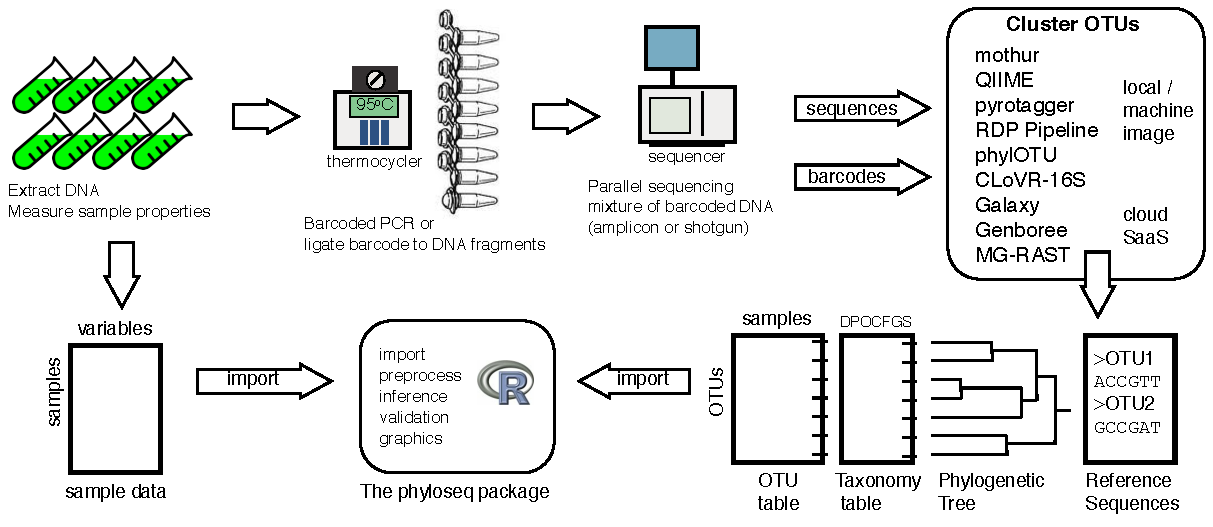
\includegraphics[width=5in]{experimental-physeq-overview-graphic.pdf}
\end{center}
\caption{
{\bf Example of a phylogenetic sequencing workflow.}
A diagram of an experimental and analysis workflow 
for amplicon or shotgun phylogenetic sequencing. 
The intended role for phyloseq is indicated.}
\label{fig:phyloSeqOverview}
\end{figure}


\subsection*{The phyloseq Project}
Many of the previously mentioned OTU-clustering applications
also perform additional downstream analyses
(Supporting Information File~S\ref{supp:comparison}).
However, typically an investigator must port
the human-unreadable output data files to other software for 
additional processing and statistical analysis 
specific to the goals of the investigation.
The powerful
statistical,
ecological,
and graphics
tools available in \R{}~\cite{Rlanguage}
make it an attractive option for this post-clustering stage of analysis.
While the computational efficiency of compiled languages like
${C^{++}}$~\cite{cpp}
make them appropriate for the expensive
but well-defined requirements of the initial sequence-processing,
the subsequent analysis is vaguely-defined and project specific;
requiring instead a broad set of interactive calculations
that is often less computationally expensive
and for which \R{} is well-suited~\cite{chambers2008}.
The public repositories of open-source \R{} extensions
(``packages'' or ``libraries'')
include many dedicated ecology and phylogenetic packages. 
For instance, there are several dozen packages listed in the CRAN Ecology Task View~\cite{CRANTV-ecology},
as well as 
distory~\cite{distorypackage}, 
phangorn~\cite{Schliep:2011hh}, 
picante~\cite{Kembel:2010ft}, 
and now phyloseq~\cite{phyloseqPSB}. 
Furthermore, \R{} includes infrastructure
for documenting an analysis in such a way
that it can be easily reproduced and modified by peers~\cite{Sweave,knitr}.

In spite of all of these highly relevant tools, 
we recently described the lack of a satisfactory standard within
\emph{Bioconductor}~\cite{Bioconductor} (or \R{} generally) for 
importing the data files from the most popular OTU-clustering applications,
or representing this data in a complete, integrated class~\cite{phyloseqPSB}.
One Bioconductor package, 
OTUbase~\cite{Beck:2011dc},
pursues some of these goals,
but has no support for phylogenetic trees in its data class,
nor support for importing data from popular/recent
OTU-clustering output formats~\cite{OTUbase-pkg,Beck:2011dc}
(Supporting Information File~S\ref{supp:comparison}).
We have proposed a new Bioconductor package,
phyloseq
(from ``\underline{phylo}genetic \underline{seq}uencing''),
dedicated to the object-oriented representation and analysis of
phylogenetic sequencing data in R~\cite{phyloseqPSB},
and supporting common OTU-clustering output formats like
QIIME~\cite{caporaso2010qiime},
mothur~\cite{mothur},
the RDP-pipeline~\cite{Cole:2009dm},
Pyrotagger~\cite{Kunin:2010wd},
and the biom-format~\cite{McDonald:2012tk}.

In this article we describe the conceptual framework and toolbox
of a substantially enhanced phyloseq codebase,
including especially some advanced ordination and graphics capabilities.
We further note that data imported by phyloseq
is also accessible to analyses encoded by
a large number of freely available \R{} packages,
in addition to the capabilities directly supported by phyloseq itself.
We will end by discussing
the notion of ``reproducible research''
in the context of phylogenetic sequencing data,
and how phyloseq and \R{} can be used
in analyses that are more open and reproducible
than those found in recent common practice.

%%%%%%%%%%%%%%%%%%%%%%%%%%%%%%%%%%%%%%%%%%%%
% You may title this section "Methods" or "Models". 
% "Models" is not a valid title for PLoS ONE authors. However, PLoS ONE
% authors may use "Analysis" 
%%%%%%%%%%%%%%%%%%%%%%%%%%%%%%%%%%%%%%%%%%%%
\section*{Methods}

\subsection*{phyloseq Project Key Features}
The phyloseq package
provides an object-oriented programming infrastructure
that simplifies many of the common data management and preprocessing tasks
required during analysis of phylogenetic sequencing data. 
This simplified syntax helps
mitigate inconsistency errors 
and encourages interaction 
with the data during preprocessing.
The phyloseq package also provides
a set of powerful analysis and graphics functions, 
building upon related packages available in \R{} and Bioconductor.
It includes or supports
some of the most commonly-needed ecology and phylogenetic tools,
including a consistent interface
for calculating ecological distances
and performing dimensional reduction (ordination).
The graphics functions allow users to interactively produce
annotated publication-quality graphics
in just one or two lines of code.
The phyloseq package includes extensive documentation
in the form of 
function- and package-level manuals embedded
in the package's documentation interface
and in a PDF version on Bioconductor~\cite{phyloseq:man:link},
as well as 
extended reproducible examples on the phyloseq homepage~\cite{phyloseq:github},
and open collaborative development on GitHub~\cite{phyloseq:github}.

\subsection*{Implementation}
The phyloseq package
adheres to the requirements for
standard \R{} packages set forth in the official
``Writing \R{} Extensions'' manual~\cite{Rext}. 
It also satisfies additional requirements
of the Bioconductor Repository~\cite{Bioconductor},
and uses a literate-programming framework based on 
structured in-source comments,
called roxygen2~\cite{roxygen2},
for (re)building the \R{} documentation (\code{.Rd}) files
and the namespace specifications.
The phyloseq package can be installed
on any system on which \R{} is supported, 
including Mac OS X, Windows, and most Linux distributions.

\subsection*{Data Availability}
\R{} packages can include example data
that is documented with the same help system
as other package objects~\cite{Rext}.
This data becomes available in the \R{} session
by invoking the \code{data} function
after the package has been loaded.
Unless otherwise noted, 
the examples provided in this manuscript use
example data that is included in the phyloseq package.


\subsection*{Data Infrastructure and Design}\label{sec:datainfrastructure}

\begin{figure}[!htbp]
\begin{center}
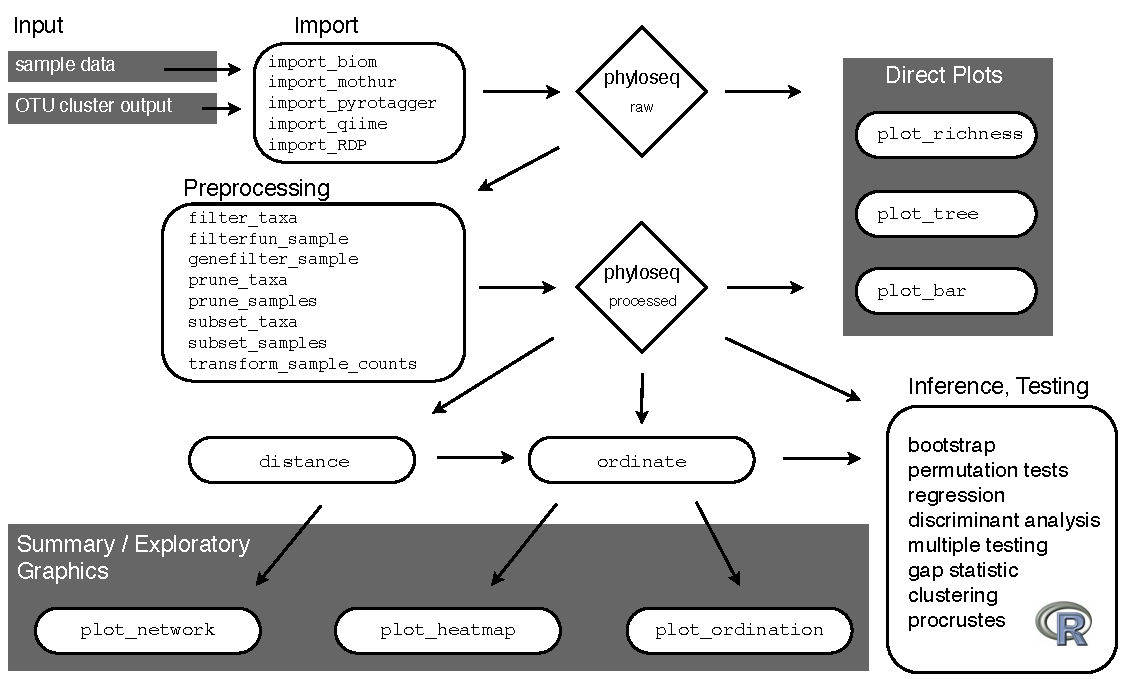
\includegraphics[width=0.9\textwidth]{phyloseq-summary-fig.pdf}
\end{center}
\caption{
{\bf Analysis workflow using phyloseq.}
The workflow starts with 
the results of OTU clustering and independently-measured sample data
(Input, top left),
and ends at various analytic procedures available in \R{}
for inference and validation.
In between are key functions for preprocessing and graphics.
Rounded rectangles and diamond shapes represent
functions and data objects, respectively,
further described in Figure~\ref{fig:phyloseqBaseClasses}.
}
\label{fig:phyloseqOverview}
\end{figure}

The phyloseq project includes an object-oriented class
that integrates the heterogeneous components of
OTU-clustered phylogenetic sequencing data.
Although Bioconductor provides many utilities
for efficient manipulation of DNA sequences, 
phyloseq does not currently re-implement 
any methods for DNA sequence
decoding, processing, or OTU-clustering
(Figure~\ref{fig:phyloSeqOverview}, Supporting Information File~S\ref{supp:comparison}). 
Instead, phyloseq provides tools to read the output files
of the most common OTU-clustering applications~\cite{caporaso2010qiime,mothur,Cole:2009dm,Kunin:2010wd},
and represents this data in \R{}
as an instance of the main data class.
This multi-component ``experiment-level'' class ---
named ``\code{phyloseq}'', and referred to here as ``the phyloseq-class''
--- 
is a key design feature of the phyloseq project,
with subsequent user-accessible functions
expecting to operate on an instance of this
class as their sole or primary input data.
These functions are described in detail
in the phyloseq manual~\cite{phyloseq:man:link},
and are part of a modular workflow
summarized in Figure~\ref{fig:phyloseqOverview}.

Figure~\ref{fig:phyloseqBaseClasses} summarizes the structure
of the phyloseq-class and its components.
Each of the slots are empty (\code{NULL}) by default,
although an instance missing an \code{otu{\_}table} component is invalid.
Tools in phyloseq that truncate dimensions of one component
(that is, remove samples or OTUs)
automatically propagate the change across all relevant components.
In general, researchers only need to manipulate their
``experiment-level'' object, 
making data (pre)processing less prone to mistakes, 
and often simplifying analysis commands to just one data argument.

\begin{figure}[!htbp]
\begin{center}
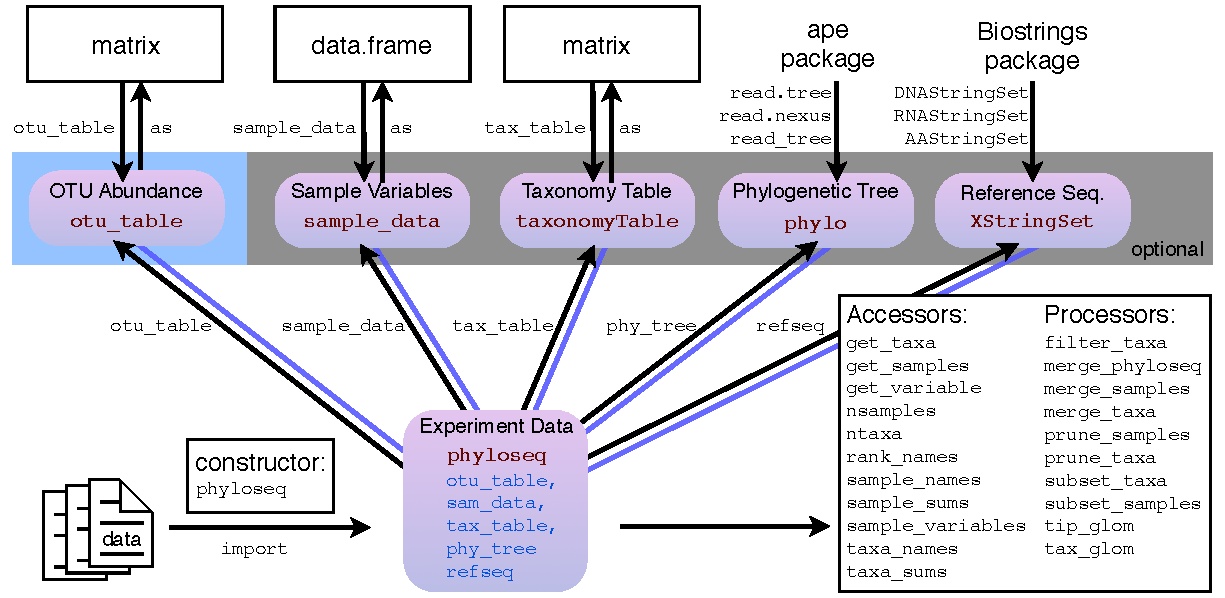
\includegraphics[width=\textwidth]{phyloseq_classes_7.pdf}
\end{center}
\caption{
{\bf The ``phyloseq'' class.}
The phyloseq class is an experiment-level
data storage class defined by the phyloseq package
for representing phylogenetic sequencing data.
Most functions in the phyloseq package
expect an instance of this class as their primary argument.
See the phyloseq manual~\cite{phyloseq:man:link}
for a complete list of functions.
}
\label{fig:phyloseqBaseClasses}
\end{figure}


\subsection*{Analysis Functions}
Complementing the data infrastructure,
the phyloseq package provides a set of functions
that take a phyloseq object as the primary data,
and performs an analysis and/or graphics task.
Figure~\ref{fig:phyloseqOverview} summarizes
the general workflow within phyloseq,
and lists some of the main functions/tools.

Comparisons of the type and quantity of
OTUs observed between microbiome samples (``beta diversity'')
is often approached through the calculation of
pairwise ecological distances~\cite{Faith:1987wx,Anderson:2006fs},
and through dimensional reduction (ordination) methods.
The phyloseq package provides a consistent interface
for the most common approaches to
distance calculations and ordination.
This interface is also the foundation for
the custom ordination and heatmap graphics functions
described in the next subsection.

In phyloseq the interface for ecological distance calculations is
a single function, \code{distance}, 
that takes a phyloseq object as its data argument
as well as a character string indicating the distance method, 
with explicit support for more than 40 ecological distance methods.
This includes a \R{}-native, optionally-parallel implementation
of Fast UniFrac~\cite{Hamady:2009}
(both weighted~\cite{Lozupone:2007kg} and unweighted~\cite{Lozupone:2005unifrac}). 
The output is a ``\code{dist}'' class distance matrix (lower-triangle)
appropriate for standard clustering analysis in core \R{} (e.g. \code{hclust}),
as well as certain dimensional reduction (ordination) methods. 

The interface for performing ordination methods is also a single function,
called \code{ordinate}, 
that takes a phyloseq object as its primary data argument
and a character string indicating the desired ordination method. 
For example, the following would perform
(unconstrained) correspondence analysis on
the included ``Global Patterns'' dataset~\cite{globalpatterns}.
\begin{knitrout}
\definecolor{shadecolor}{rgb}{1, 1, 1}\color{fgcolor}\begin{kframe}
\begin{alltt}
\hlfunctioncall{data}(GlobalPatterns)
gp_ord_ca = \hlfunctioncall{ordinate}(GlobalPatterns, \hlstring{"CCA"})
\end{alltt}
\end{kframe}
\end{knitrout}


The \code{ordinate} function currently supports
correspondence analysis (CA)~\cite{Greenacre:1984}, 
constrained correspondence analysis (CCA)~\cite{Braak:1986fr}, 
detrended correspondence analysis (DCA)~\cite{Hill:1980wk}, 
redundancy analysis (RDA)~\cite{Wollenberg:1977im}, 
principal components analysis (PCA)~\cite{Hotelling:1933ki}, 
double principle coordinates analysis (DPCoA)~\cite{Pavoine:2004}, 
multidimensional scaling (MDS, PCoA)~\cite{gower:1966hi}, 
and non-metric multidimensional scaling (NMDS)~\cite{Minchin:1987fl}. 
For CA, CCA, DCA, RDA, and DPCoA,
the ordination is based upon an evaluation of abundance values
(in the case of DPCoA, the patristic distances between OTUs
on the phylogenetic tree is also used), 
but not an ecological distance.
For MDS and NMDS, the \code{ordinate} function requires
a pre-calculated distance matrix (``\code{dist}'' object)
or the name of a supported ecological distance method.
For example, PCoA/MDS can be calculated on
an unweighted UniFrac distance matrix~\cite{Lozupone:2005unifrac}, 
using the following command:

\begin{knitrout}
\definecolor{shadecolor}{rgb}{1, 1, 1}\color{fgcolor}\begin{kframe}
\begin{alltt}
gp_mds_uf = \hlfunctioncall{ordinate}(GlobalPatterns, \hlstring{"MDS"}, \hlstring{"unifrac"})
\end{alltt}
\end{kframe}
\end{knitrout}


There are many combinations of approaches possible
(even extending into time-series of table pairs),
and the optimal approach depends on the goals of the experiment
and characteristics of the data~\cite{Thioulouse2011}.
The phyloseq package also includes a specialized function
for displaying ordination results in different ways,
described in the following section.

\begin{figure}[!htbp]
\begin{center}
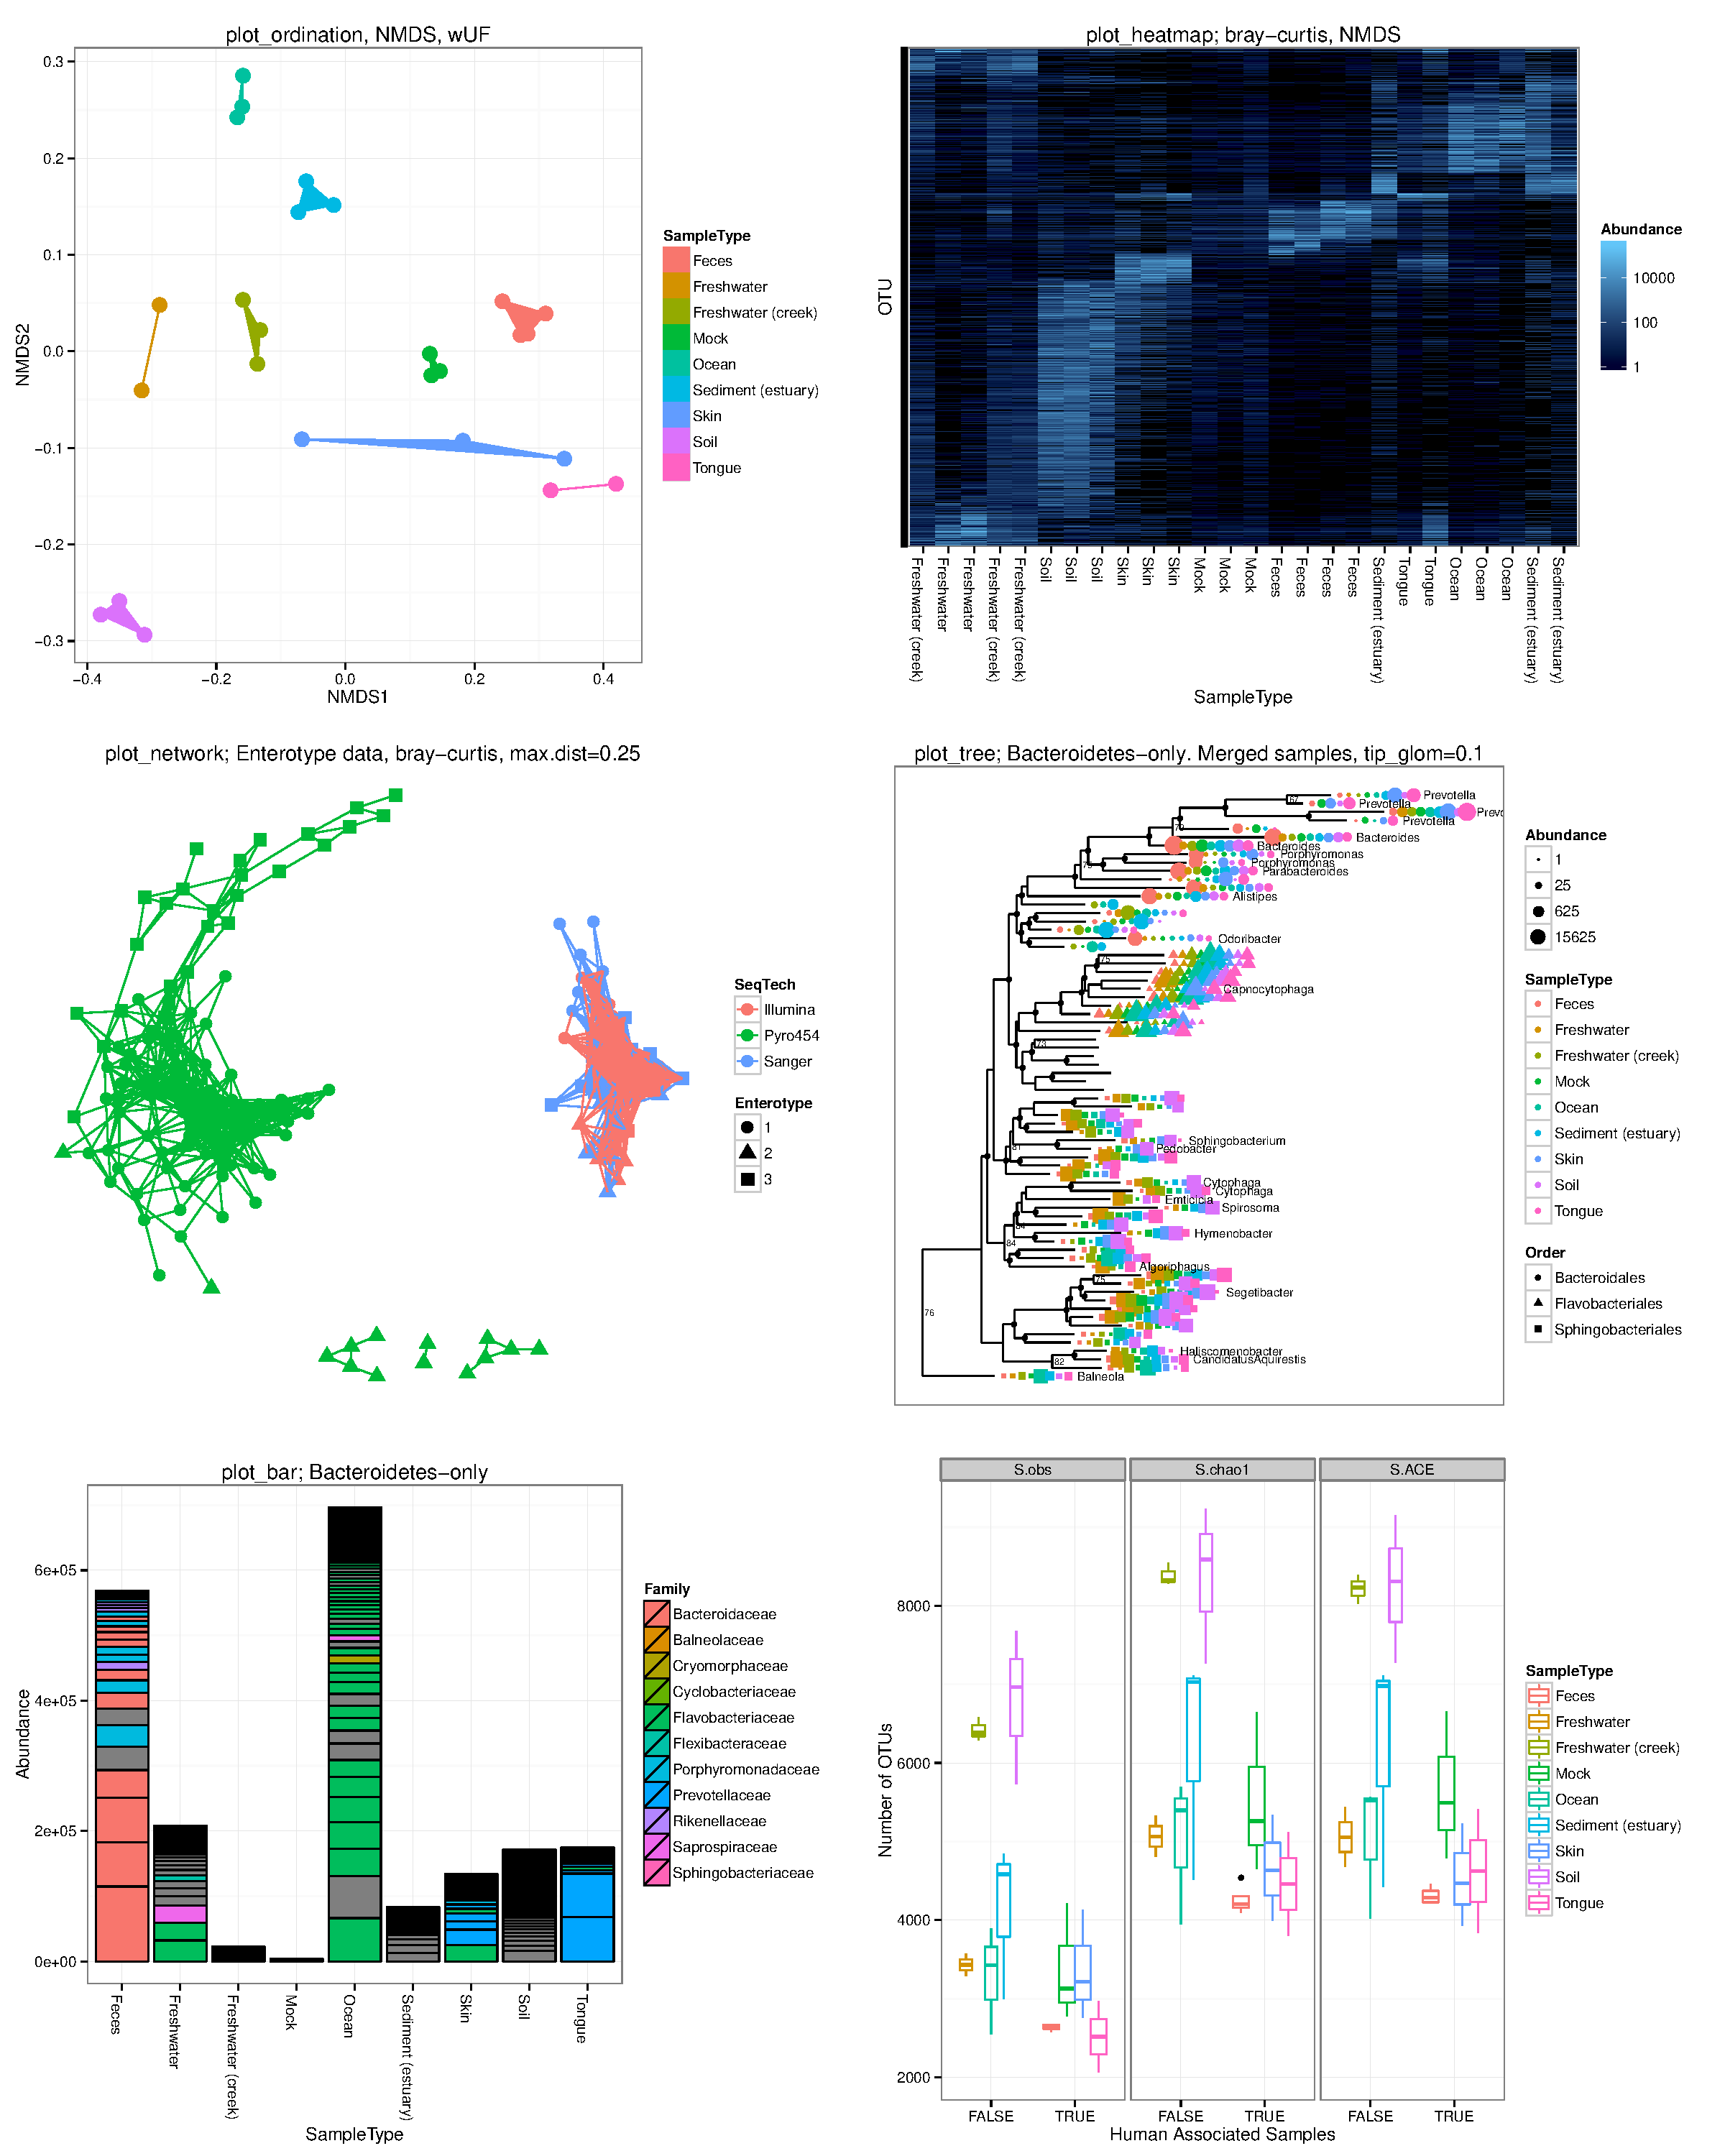
\includegraphics[width=\textwidth]{submit-main/phyloseq-plot-main.pdf}
\end{center}
\caption{
{\bf Different graphic summaries of \emph{Global Patterns} data
using the phyloseq package.}
The \emph{Global Patterns} data was provided by the authors~\cite{globalpatterns},
and is included in phyloseq as an example dataset.
Prior to plotting,
each sample was transformed to the same total read depth, 
and OTUs were trimmed that were not observed at least 3 times in 20\% of samples or had a coefficient of variation $\leq{}3.0$ across all samples. 
For the \code{plot{\_}tree} and \code{plot{\_}bar} subplots,
only the Bacteroidetes phylum is shown.
Each subplot title indicates the plot function that produced it.
The \R{} script completely reproducing this figure 
(including preprocessing)
is provided in Supporting Information File~S\ref{supp:sweave:source}.
All of these functions return a \code{ggplot} object
that can be further customized/modified
by tools in the ggplot2 package~\cite{ggplot2}.
See additional descriptions of each function in the body text,
and at the phyloseq homepage~\cite{phyloseq:github}.
}
\label{fig:phyloseqPlot}
\end{figure}


\subsection*{Specialized Graphics}\label{sec:graphics:functions}

One of the key features of the phyloseq package
is a set of graphics functions custom-tailored
for phylogenetic sequencing analysis,
built using the ggplot2 package~\cite{ggplot2}.
The ggplot2 package is an implementation
of Wilkinson's \emph{The Grammar of Graphics},
which provides an object-oriented description
of analytical graphics that emphasizes
the separation of data
and its mapping to aesthetic attributes~\cite{Wilkinson:GoG}.
In the phyloseq package,
functions having names beginning with ``\code{plot{\_}}''
require a phyloseq object as input data,
and return a ggplot2 graphics object.
These \code{plot{\_}} functions support optional mapping
of color, size, and shape aesthetics
to sample or OTU variables ---
usually by providing the name of
the variable or taxonomic rank
as a character string
(E.g. \code{color =}``\code{SampleType}'').
Legends are automatically generated
based on the data and aesthetic mappings
(not true of the base \R{} graphics),
and all features of these graphics
can be further modified in \R{}
via functions/options in the ggplot2 package.

The following list summarizes the key graphics-producing functions in phyloseq,
which are also demonstrated in Figure~\ref{fig:phyloseqPlot},
and in phyloseq's online tutorials~\cite{phyloseq:github}.
Supporting Information File~S\ref{supp:sweave:source} provides the complete R code for creating Figures~\ref{fig:phyloseqPlot} and~\ref{fig:plot:ordination}.
We have also included some additional examples
of graphics created by \code{plot{\_}ordination}
(Figure~\ref{fig:plot:ordination}).
They emphasize different aspects of ordination results, 
and the best choice depends heavily
on characteristics of the data
and research questions.
The provided code also demonstrates
a custom modification to the ggplot2 graphic,
in this case the addition of a two-dimensional density estimate
to the ``OTUs-only'' plot
(Supporting Information File~S\ref{supp:sweave:source}).


\begin{enumerate} 
\item \code{plot{\_}ordination}.
This is the main function for plotting the results of an ordination.
It currently supports four different representations of the ordination results:
samples-only,
OTUs-only,
``biplot'' (combined) representation,
and ``split''.
A demonstration of these different options
is provided in Figure~\ref{fig:plot:ordination}.
As can be seen in these examples,
the ``biplot'' and ``split'' options support dual projections
of both OTU- and sample-space.
Additional parameters easily map 
the respective sample variable or taxonomic rank
to color, size, or shape aesthetics.

\item \code{plot{\_}heatmap}.
This is a special implementation of the ordination-organized heat map
similar to the NeatMap package~\cite{neatmap}.
Briefly, the abundance matrix is represented as a grid of colored tiles,
with the color of the tiles mapped to the
(usually transformed) abundance value.
The ordering of the OTUs and sample indices in this representation
is critical for discriminating any patterns.
Traditionally, hierarchical clustering methods
have been used for this organization; 
but, as Rajaram and Oono recently pointed out~\cite{neatmap},
this has the potential to misrepresent the data
when deeply-branching elements are placed next to one another arbitrarily.
Instead, the samples (and optionally, OTUs) are reordered
based on their radial coordinate angle
in the first two axes of an ordination.
For the \code{plot{\_}heatmap} function,
any of the distances/ordinations supported by
the \code{distance} and \code{ordinate} functions
can be used,
with the default being non-metric multidimensional scaling.
Any arbitrary color scale can be selected,
as well as any choice of numerical transformation
for scaling the mapping of color shades to abundance.

\item \code{plot{\_}network}.
This function plots an igraph-class network~\cite{igraph}
representing binary relationships between samples or OTUs.
The network is calculated using the \code{make{\_}network} function
with phyloseq data as input and a desired ecological distance and threshold value.
Unlike ordination, where most of the data structure is summarized
by the relative position in two or more axes, 
the data is instead summarized by connections
between samples (or OTUs) drawn with straight lines.
Two samples are considered ``connected'' if the distance between them
is less than a user-defined threshold.
The relative position of points is optimized
for the visual display of network properties,
but is otherwise arbitrary.
Any of the ecological distances supported by the \code{distance} function
can be selected,
and this can be a powerful representation of major clusters among samples or OTUs,
provided the value of the distance threshold has been chosen carefully.

\item \code{plot{\_}tree}.
This function facilitates easy graphical rendering/investigation
of the phylogenetic tree, with sample data overlaid.
In some cases an annotated tree
can be a powerful representation
of an underlying evolutionary structure.
The \code{plot{\_}tree} function
optionally places successive points next to the tips of the tree,
indicating the samples in which each OTU was observed.
These points can have their color, shape, and size aesthetics
mapped to sample variables,
revealing the correspondence of
environmental variables on specific regions 
of the evolutionary tree.
Standard ggplot2 customizations are supported, 
and this is, to our knowledge, the only function
for ggplot2-based phylogenetic trees
currently available 
in the CRAN/Bioconductor repositories.
For phylogenetic sequencing of samples with large richness,
some of the options in this function will be
prohibitively slow to render or too dense to be interpretable,
a drawback to summarizing
phylogenetic sequencing data using trees.
One suggestion is to either agglomerate or subset the data
such that there are not more than 200 or so OTUs (tree tips) on a given plot,
sometimes less depending on the complexity
of the additional annotations being mapped to the tree.
In many modern datasets 200 OTUs (or less) will be insufficient
to summarize the entire dataset,
in which case one or more of the other plot methods is suggested.

\item \code{plot{\_}bar}.
Although sometimes very complicated, 
a well-organized bar plot can be an effective graphical means
for direct quantitative comparison of abundance values,
and we note that statisticians generally discourage
the use of pie-charts~\cite{Tufte:1983vw}.
The \code{plot{\_}bar} function
takes as input a phyloseq dataset and 
a collection of arbitrary expressions
for grouping the data based upon
taxonomic rank and sample variables.
The returned graphic represents each abundance value
as the height of a rectangular block
that is outlined by a thin black line
and filled with the corresponding color of
the user-specified sample or taxonomic variable, grey by default.
Each of these OTU abundance rectangles corresponding to
the same horizontal position (usually sample, or sample group)
are stacked in order of abundance,
such that the aggregate height of the stacked bar
is also quantitatively informative. 

\item \code{plot{\_}richness}.
This function creates plots of richness estimates
of each sample in a phyloseq data object,
allowing for horizontal grouping and color shading
according to additional sample variables.
Differences in richness (alpha diversity) between samples
is often one of the first questions asked 
of phylogenetic sequencing data.

\end{enumerate} 

\FloatBarrier


\begin{figure}[!htbp]
\begin{center}
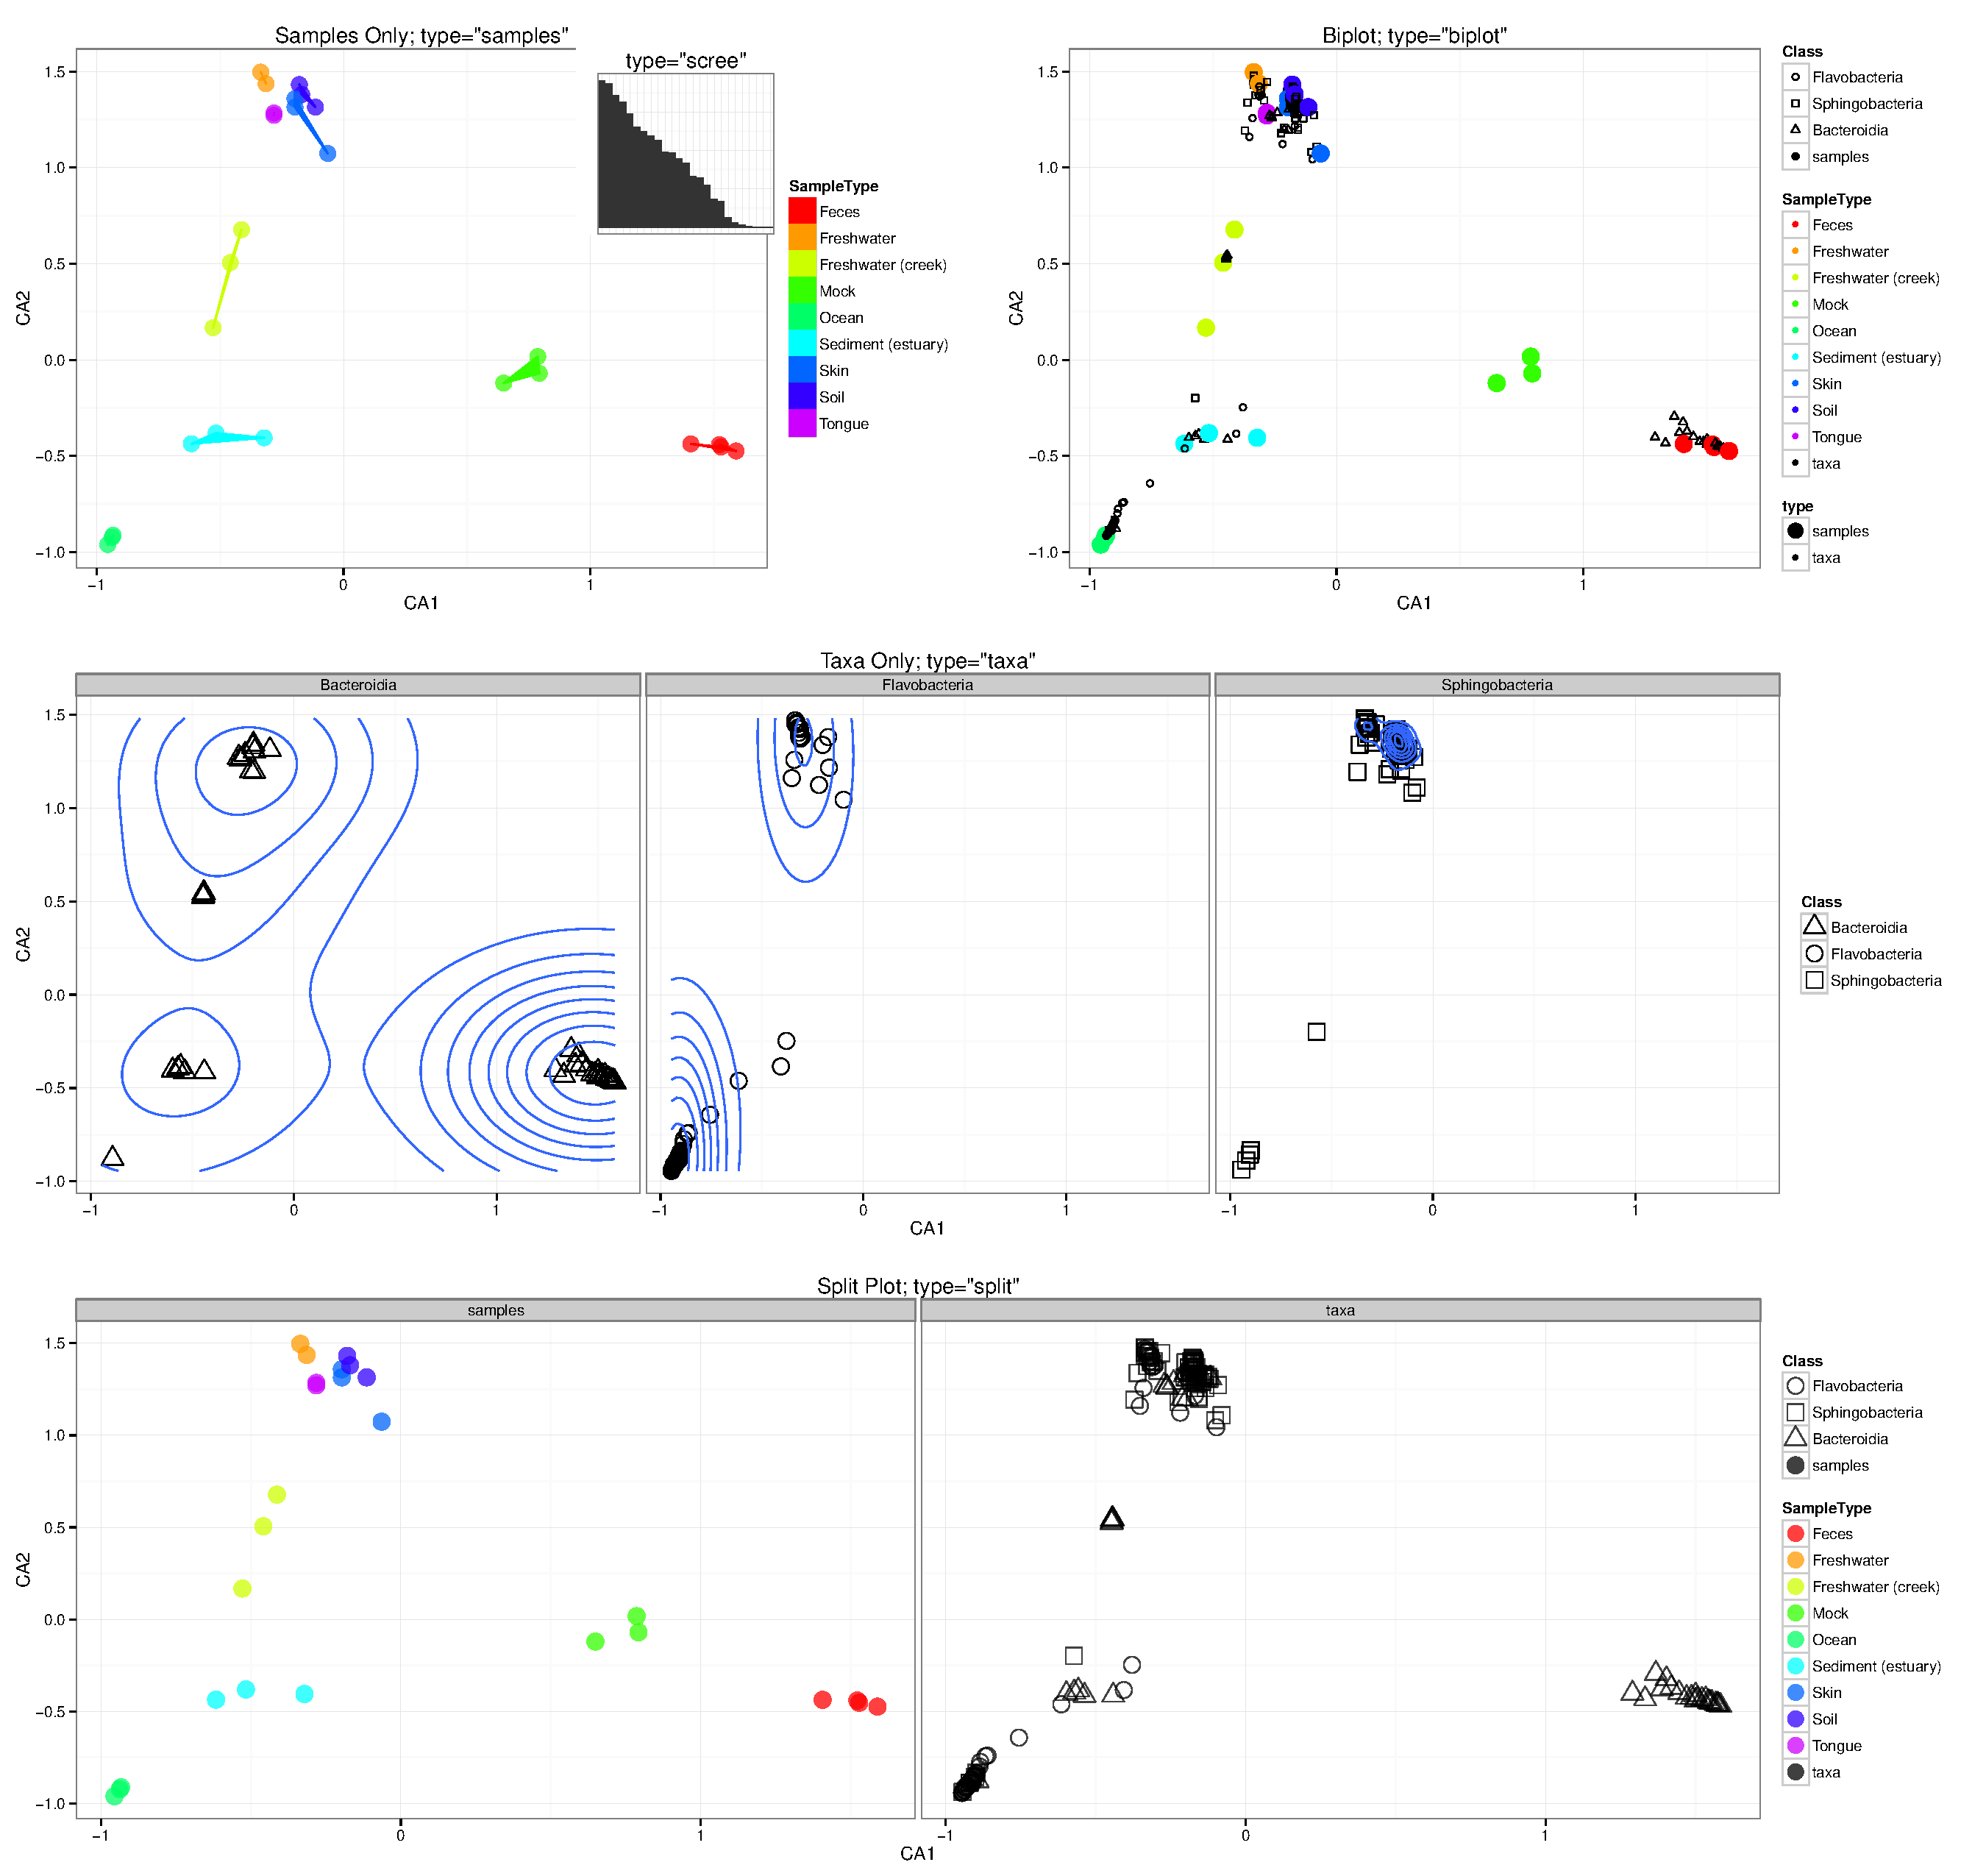
\includegraphics[width=\textwidth]{submit-main/phyloseq-plot-ordination.pdf}
\end{center}
\caption{
{\bf \code{plot{\_}ordination} display methods included in phyloseq.}
Each panel uses a ``Bacteroidetes-only" subset
of the preprocessed ``Global Patterns'' dataset
that was also used in Figure~\ref{fig:phyloseqPlot}.
The coordinates are derived from
an unconstrained correspondence analysis~\cite{greenacre2007}.
Different panels illustrate different displays
of the ordination results using the \code{type} argument
to the \code{plot{\_}ordination} function.
(Top Left) Example of a samples-only display,
with the ``SampleType'' mapped to the color aesthetic,
and a filled-polygon layer to emphasize plot regions
where sample types co-occur. 
(Top Left Insert) A ``scree'' plot of the eigenvalues
associated with each axis,
which indicates the proportion of total variability
represented in each axis. 
(Top Right) Biplot representation in which
samples and OTUs ordination results are overlaid.
Clumps of OTUs appear to co-occur with different sample types,
and some correlation with taxonomic phylum is also evident.
(Middle) An OTUs-only plot that has been faceted
(separated into panels) by class,
with a two-dimensional density estimate overlain in blue.
This view shows clearly a lack of association
between the Sphingobacteria and Flavobacteria classes
with fecal samples,
which appear to be enriched in a subset of the Bacteroidia
(relative to other OTUs in this Bacteroidetes-only dataset).
Meanwhile, subsets of Bacteroidia appear to be enriched
within multiple sample types.
(Bottom) The ``split'' type for this graphic, 
in which both samples-only and OTUs-only plots are created,
and shown side-by-side with one legend and shared vertical axis.
Both the ``biplot'' and ``split'' options allow dual projections
of both OTU- and sample-space.
}
\label{fig:plot:ordination}
\end{figure}

\FloatBarrier

\subsection*{Normalization and Standardization}
In multivariate analyses such as PCA, 
large differences in variances between columns are corrected
by standardizing each column; 
i.e. dividing each column by its standard deviation.
Thus each column will have the same weight in the multivariate analysis.
For OTU abundance tables, such a procedure is inappropriate
as the disparities in column sums can be 100-fold.
Methods based on chi-squared distances 
rather than variances deal with this
by comparing weighted column profiles~\cite{greenacre2007},
computed as relative abundances
for each OTU within a column, with the overall column sum
retained as a weighting factor. 
However, chi-square distances are sums of squares 
and can be overly sensitive
to outliers and sequencing ``jackpot'' effects
such as those occurring in pyrosequencing data~\cite{Pinto:2012bk}.
Bray-Curtis distances can be a useful alternative, 
as it is based on the $L^1$ distance between profiles,
as long as the differences in actual column sums 
are also accounted for in the final study.
The other approach to the problem
of disparities between column sums
has been to subsample the over-abundant columns
down to the same number as the smaller ones.
However this results in a loss of information,
rarely an optimal procedure in statistical contexts.
This subsampling procedure is inspired by the popular idea of rarefaction 
in coverage studies first invented by Sanders~\cite{Sanders:1968},
but has yet to be proved beneficial for all microbial community structures.
The parallels between gene expression microarray analyses
and microbial abundance analyses
was mentioned in~\cite{Holmes:2011vb},
which proposed several expression-inspired strategies 
for robustifying abundance measurements.
The main points were that rankings and thresholding are important
in the presence of noise and high variability in sequence depths.
As in gene expression analysis filtering the OTUs is beneficial,
especially in the latter multiple testing adjustments.
The phyloseq package enables easy filtering and rank transformations
in the same vein as robust multi-array averaging (rma)~\cite{Allison:2006fk}.
We provide further details in (McMurdie and Holmes,~\cite{holmes:pnas:ch7}).

\FloatBarrier

\subsection*{Confirmatory Analyses}
Although useful for exploring and summarizing microbiome data,
many of the graphics and ordination methods discussed here
are not formal tests of any particular hypothesis. 
The most common framework for testing in microbiome studies 
is the comparisons of samples from different categories
(e.g. healthy and obese; control and treated; different environments). 
Standard test statistics include the
t-test, 
the paired permutation t-test, 
and ANOVA type tests based on F or pseudo-F statistics.
However, microbiome data have two particularities.
First, the raw abundance counts are never normally distributed,
so the preferred methods are nonparametric.
Second, there is contiguous information available 
about the relationships between OTUs,
as well as for variables measured on the samples,
so testing is sometimes more elaborate
than a two-sample test.
The hypergeometric test,
also known as Fisher's exact test,
is used in cases when we have a test statistic for each
of the different OTUs.
The goal is to confirm that a certain property of these significant
OTUs is overrepresented compared to the general population of OTUs,
often called ``the universe''.
For instance
in Holmes et al~\cite{Holmes:2011vb}
and Nelson et al~\cite{Nelson:2010}
several phyla were shown to be significantly over-abundant 
in IBS rats as compared to healthy controls using this hypergeometric test. 

An organizing principle in many nonparametric 
testing protocols is that the repetition
of an analysis multiple times
enables the user to control for multiple testing, 
or to evaluate the quality of estimators 
or the optimal values of tuning parameters.
Modern confirmatory analyses currently depend 
on these repeated analyses under various
data perturbation schemes,
of which
resampling, 
permutations,
and Monte Carlo simulations are the most common. 
For instance the bootstrap uses
many thousands of analyses of resampled data
to address problems such as
statistical stability or
bias estimation~\cite{efron1993introduction},
and can even provide confidence regions~\cite{efron1993introduction}
for nonstandard parameters, such as phylogenetic trees~\cite{holmes2003bootstrapping}.
Repeating analyses on permuted data
can allow for control of the probability
of encountering 1 or more false positives (falsely rejected nulls)
among your group of simultaneous hypotheses, 
also called the Family Wise Error Rate (FWER).
For instance, Westfall and Young's permutation-based \textbf{minP} procedure
controls the FWER~\cite{Westfall:1993uu}
and is implemented within the multtest package~\cite{multtest}.
The phyloseq package interfaces with minP in multtest
through a wrapper function, called \code{mt}.
In the following example code we use the \code{mt} wrapper
to control the FWER while simultaneously testing
whether each OTU correlates with
the ``Enterotypes'' classification of the samples.
Note that we first remove samples
that were not assigned an enterotype by the original authors
(Table~\ref{tab:entmt}).

\begin{knitrout}
\definecolor{shadecolor}{rgb}{1, 1, 1}\color{fgcolor}\begin{kframe}
\begin{alltt}
\hlfunctioncall{data}(enterotype)
x = \hlfunctioncall{subset_samples}(enterotype, !\hlfunctioncall{is.na}(Enterotype))
\hlfunctioncall{head}(\hlfunctioncall{mt}(x, \hlstring{"Enterotype"}, test = \hlstring{"f"}), 8)
\end{alltt}
\end{kframe}
\end{knitrout}



%%%%%%%%%%%%%%%%%%%%%%%%%%%%%%%%%%%%%%%%%%%%%%%%%%%%%%%%
% Results and Discussion
%%%%%%%%%%%%%%%%%%%%%%%%%%%%%%%%%%%%%%%%%%%%%%%%%%%%%%%%
\section*{Results and Discussion}
As the complexity and sophistication
of phylogenetic sequencing experiments continues to increase,
it is clear that a ``one-analysis fits all'' approach is not sufficient.
While it is often useful and convenient to have common analyses 
coupled within the application that decodes the sequences and clusters OTUs,
we posit that a separate set of 
flexible open-source analytical tools is also needed 
that can be reproduced consistently by peers,
and easily applied to new datasets and data sources.
It should include a large library of statistical functions, 
and be independent of the choice of 
OTU-clustering method or sequencing technology.
The phyloseq package helps satisfy this need by
reducing the effort necessary to analyze
OTU-clustered phylogenetic sequencing data
via the \R{} language and interactive computing environment.


%%%%%%%%%%%%%%%%%%%%%%%%%%%%%%%%%%%%%%%%%%%%
% Reproducible Research.
%%%%%%%%%%%%%%%%%%%%%%%%%%%%%%%%%%%%%%%%%%%%

\subsection*{Reproducible Research and Sharing}

In exploratory statistical work
it is easy to produce biased results~\cite{Ioannidis:2005bw}
through poorly chosen metrics or tests, 
a failure to properly control for multiple inferences,
undisclosed data ``pruning'', 
and probably many other means.
Although not commonly required~\cite{Merali:nature:2010,Peng02122011,Ince:2012iy},
an important defense against biased (or poorly-supported) findings
is a higher standard for reproducibility in published research~\cite{Carey:2010gq},
in which journal articles are accompanied by sufficient data and software
such that all presented analyses, tables, and figures
can be reproduced exactly and with minimal effort~\cite{Peng02122011}.
In this context of highly-parallel phylogenetic-sequencing experiments,
reproducible research can be partially facilitated by
emerging standards
for experimental design~\cite{Knight:2012gf}
and file format~\cite{McDonald:2012tk}.
Virtual machine image and cloud-deployed
``pipeline'' analyses~\cite{caporaso2010qiime,Angiuoli:2011ib,Meyer:2008db}
can further increase accessibility of analyses by mitigating
the need for expensive computing hardware
while also avoiding complicated installation procedures.
However, the use of publicly available ``pipeline'' tools 
does not fully meet the reproducibility standard
unless accompanied with the complete code and data used
in the analysis being published~\cite{Peng02122011}.
This is especially important when considering the many choices
that are involved in decoding, OTU-clustering, and preprocessing;
as well as the many varied approaches to
incorporating sample covariates
and performing multivariate analyses on complex data.
The recent release of the HMP data and multiple articles on the results
from their analyses underscore this fact.
Thresholding and noise filtering
were done independently by each team, 
but no overall robustness study was performed~\cite{HMPC:2012bb}.
Changes early in the analysis pipeline could have downstream effects
that are now prohibitively difficult or impossible to evaluate.
Generally speaking, the preprocessing of OTU abundance data 
through filtering, normalizing, centering, shrinking, and other transformations
is a common practice and necessary for analysis~\cite{Allison:2006fk}, 
but varies widely among researchers 
and is often difficult to reproduce.
This is particularly true when the preprocessing transformations are the result of 
``manual'' adjustments in a spreadsheet, 
custom code/script that is not included in the publication,
or random subsampling (``rarefying'' to even sequencing effort)
with no reported seed.
A related example is the (often not-so) reproducible choice of tuning parameters
and perturbation-based statistical validation procedures,
allowing for the easy testing of alternatives and robustness of results.
To a large extent this revisits many of the same issues
of reproducible research~\cite{Donoho:2010cx,Peng:2009jy,Gentleman:2004vk} 
that have been addressed over the last decade
for the analysis of microarray data~\cite{Allison:2006fk},
and for which there are many proven tools already available in Bioconductor/\R{}. 
The emphasis of preprocessing tools in phyloseq
is intended to decrease the extent to which these steps constitute
opaque and idiosyncratic efforts by investigators,
while making the results of different studies more comparable.

One of the goals of the phyloseq project is to help close
the gap in reproducible research that presently exists
between pipeline results
and the additional analyses required by investigators.
This can be achieved when phyloseq is used
(possibly with other \R{} packages) 
in conjunction with documentation tools such as 
Sweave~\cite{Sweave},
knitr~\cite{knitr},
iPython~\cite{ipython} Notebook invoking the rmagic extension,
or ``\R{} flavored markdown'' (RFM)~\cite{Rmarkdown}.
The Sweave-format approach
is part of the reproducible research standards
strongly encouraged by the journal \emph{Biostatistics}~\cite{Peng:2009jy},
as well as many disciplines related to
statistics and bioinformatics~\cite{Carey:2010gq,Gentleman:2005jk}.
The recently-described RFM format and iPython Notebook
can also work very well
for cases where a web-browser is a satisfactory documentation delivery medium,
with RFM being our preferred source format for
publishing reproducible online tutorials
with embedded code and figures (HTML5)~\cite{phyloseq:demo,phyloseq:github}.
We emphasize that the benefits of reproducibility
are not contingent on ``pretty'' code~\cite{Barnes:2010dn},
and we encourage researchers in the field to
make their code available even if they feel
insecure about its programmatic elegance.
As an illustrative example, we have made available
the Sweave (\code{.Rnw}) and supporting files required
to completely reproduce this article,
including especially the complete source as an RFM file (\code{.Rmd})
with its associated output HTML file,
both of which provide the preprocessing steps and graphics commands needed 
to exactly reproduce each figure
(Supporting Information File~S\ref{supp:sweave:source}).
We have also published a GitHub repository dedicated to
reproducible demonstrations of analyses with phyloseq~\cite{phyloseq:demo}.


\subsection*{Extending phyloseq}
It is important to note that the new phyloseq-class
is a significant departure from 
the originally-proposed phyloseq-class structure~\cite{phyloseqPSB}, 
which used nested multiple inheritance and a naming convention. 
It was a valid approach in principle, 
but was an overly complex approach for the goal of
representing a phylogenetic sequencing experiment as a single object.
The updated phyloseq-class is simple to extend for developers
and easy to explain to users (Figure~\ref{fig:phyloseqBaseClasses}).
In general, the downstream analysis and plotting functions
that might operate on an instance of the phyloseq-class
do not need to (re)perform common validity checks 
because these checks are consolidated as part of
the phyloseq-constructor method.
      
Analysis tools available in \R{} but not explicitly wrapped in phyloseq
are nevertheless available to users and developers 
via accessors and other data infrastructure tools. 
This leverages the fact that phyloseq data components
are based on standard \R{} data classes
and easily used in other package settings in \R{}. 
For example, we have included example code that illustrates
the use of the \code{bioenv} function from the vegan package,
starting with data represented by the phyloseq-class
(See Supporting Information File S\ref{supp:sweave:source} for code,
and the phyloseq demo~\cite{phyloseq:demo}).
Similarly,
as an open-source package in an open language/framework (\R), 
phyloseq can be easily included
at the relevant steps in pipelines, workbenches, and GUIs
now under active development
(E.g. ClovR~\cite{Angiuoli:2011ib},
MG-RAST~\cite{Meyer:2008db}, 
QIIME~\cite{caporaso2010qiime}, 
mcaGUI~\cite{Copeland:2012co}).
This represents a means for investigators with limited programming literacy
to still benefit from some of the tools included in, or facilitated by, phyloseq.


%%%%%%%%%%%%%%%%%%%%%%%%%%%%%%%%%%%%%%%%%%%%
% Conclusions
%%%%%%%%%%%%%%%%%%%%%%%%%%%%%%%%%%%%%%%%%%%%
\section*{Conclusions}
The phyloseq project is a new open-source software tool
for statistical analysis of phylogenetic sequencing data
within the \R{} programming language and environment.
The tools in phyloseq make it easy to
read the data output of several of the most common
OTU clustering pipelines,
and also represents this data in a unified, integrated form
amenable to many modern analysis methods.
With this integrated representation of the data
it is easy to use supervised methods ---
such as canonical correspondence analysis,
discriminant correspondence analysis,
sparse linear discriminant analysis, etc.
---
to explain clinical or environmental response variables.
We hope that this will provide a gateway for users
to take their analyses towards more robust nonparametric alternatives
to classical least squares methods,
and allow them to interact graphically with their data
more easily and efficiently.
By leveraging existing \R{} infrastructure for reproducible research,
the phyloseq project also enables reproducible
preprocessing,
analysis,
and publication-quality graphics production ---
such that it is easy to document, share, and modify
analyses of phylogenetic sequencing data.
The phyloseq package 
is released on Bioconductor~\cite{Bioconductor}
and developed collaboratively on GitHub~\cite{phyloseq:github}.


\clearpage
%%%%%%%%%%%%%%%%%%%%%%%%%%%%%%%%%%%%%%%%%%%%
% Availability and Requirements
%%%%%%%%%%%%%%%%%%%%%%%%%%%%%%%%%%%%%%%%%%%%
\section*{Availability and Requirements}
\paragraph*{Project name:} phyloseq
\paragraph*{Project Stable Release:} \url{http://www.bioconductor.org/packages/release/bioc/html/phyloseq.html} 
\paragraph*{Project Home Page:} \url{http://joey711.github.com/phyloseq/} 
\paragraph*{Project Issue Tracker:} \url{https://github.com/joey711/phyloseq/issues} 
\paragraph*{Project Demo Page:} \url{http://joey711.github.com/phyloseq-demo/} 
\paragraph*{Operating System(s):} Platform Independent
\paragraph*{Programming Language(s):} \R{}
\paragraph*{Other Requirements:} \R{}, \R{} packages
(ade4, ape, Biostrings, foreach, ggplot2, igraph0, multtest, picante, plyr, reshape, RJSONIO, scales, vegan )
\paragraph*{License:} AGPL-3
  

% Do NOT remove this, even if you are not including acknowledgments
\section*{Acknowledgments}
  %\ifthenelse{\boolean{publ}}{\small}{}
We would like to thank Martin Morgan and Valerie Obenchain
at Bioconductor for their useful suggestions regarding
the architecture and organization of phyloseq.
We would also like to thank the developers of the open source packages
on which phyloseq depends,
in particular 
Rob Knight and his lab for QIIME~\cite{caporaso2010qiime}, 
Hadley Wickham for the ggplot2~\cite{ggplot2}, reshape~\cite{reshape}, and plyr~\cite{plyr} packages,
as well as 
the Bioconductor and \R{} teams~\cite{Bioconductor,Rlanguage}.
Thanks also to RStudio and GitHub for
immensely useful and free development applications.
Julia Fukuyama provided prototype code for the DPCoA wrapper.
Gregory Jordan provided several core functions that make a 
ggplot2-based phylogenetic tree plot possible,
borrowed with permission from his ``ggphylo'' repository.
Scott Chamberlain provided useful example code for a 
ggplot2-based network plot in his ``gggraph'' repository.
Julia Fukuyama, Sam Pimentel, Kris Sankaran and Dustin Janatpour
provided early feedback on the phyloseq package. 
Les Dethlefsen, Diana Proctor and other members of the David Relman Lab 
provided ongoing feedback and example data. 
Alfred Spormann, Tyrrell Nelson and Tim Meyer also provided
early versions of an illustrative data set. 
We also thank the communities at stackoverflow.com
for useful advice during development of phyloseq.


\clearpage
%%%%%%%%%%%%%%%%%%%%%%%%%%%%%%%%%%%%%%%%%%%%
% REFERENCES
%%%%%%%%%%%%%%%%%%%%%%%%%%%%%%%%%%%%%%%%%%%%
%\section*{References}

% The bibtex filename
\bibliography{phyloseq-plos1-2013}



\clearpage
%%%%%%%%%%%%%%%%%%%%%%%%%%%%%%%%%%%%%%%%%%%%
% Figures & Tables with captions
%%%%%%%%%%%%%%%%%%%%%%%%%%%%%%%%%%%%%%%%%%%%
\section*{Table Legends}
\begin{table}[htbp]
\centering
\begin{tabular}{lrrrr}
\hline
genera  & index & 	test stat & raw-p & 	adj-p	\\
\hline
Prevotella                &      207 &344.73 & 0.0001 & 0.0158  \\
Bacteroides               &      203 & 85.01 & 0.0001 & 0.0158  \\
Blautia                   &      187 & 19.52 & 0.0001 & 0.0158  \\
Bryantella                &      503 & 16.38 & 0.0001 & 0.0158  \\
Parabacteroides           &      205 & 12.89 & 0.0001 & 0.0158  \\
Alistipes                 &      208 &  8.71 & 0.0002 & 0.0301  \\
Bifidobacterium           &      240 &  9.29 & 0.0004 & 0.0560  \\
Holdemania                &      201 &  7.64 & 0.0009 & 0.1146  \\
\hline
\end{tabular}
\caption{
{\bf Results from the \code{mt} function on the ``Enterotypes'' dataset.}
The original ``Enterotypes'' dataset~\cite{enterotypes}
(included in phyloseq)
with OTU-wise testing of enterotype groups. 
Tests are a permutation-adjusted F-test 
using the Family-Wise Error Rate (FWER)
as correction for multiple inferences (``adj-p'' column).
Not surprisingly, \emph{Prevotella} and \emph{Bacteroides} top the list,
as they were major components of the ``Enterotypes'' classification
described in the original article~\cite{enterotypes}.
}
\label{tab:entmt}
\end{table}

\section*{Figure Legends}
%Main figure legends go here at time of submit.


%%%%%%%%%%%%%%%%%%%%%%%%%%%%%%%%%%%%%%%%%%%%
% Supplemental Information Files/Legends
%%%%%%%%%%%%%%%%%%%%%%%%%%%%%%%%%%%%%%%%%%%%
\subsection*{Supporting Information Legends}
% Remove the automatic label so that you can add it explicitly with S in front
\captionsetup{labelformat=empty, labelsep=none} 
% Re-set the figure counter
\setcounter{figure}{0}


% The software comparison table
\begin{figure}[!ht]
\begin{center}
\end{center}
\caption{
{\bf Supporting Information File~S\ref{supp:comparison}.
Summary of comparison between phyloseq and currently available software.}
This PDF file contains a table summarizing a comparison of supported capabilities between phyloseq and QIIME~\cite{caporaso2010qiime}, mothur~\cite{mothur}, and the pair of packages OTUbase~\cite{Beck:2011dc} and mcaGUI~\cite{Copeland:2012co}. 
A ``+'' or ``--'' indicates that the capability is not directly supported, respectively. A symbol or word instead of ``+'' implies that the capability is supported, but with an extra caveat or detail, further defined below the table, if necessary. This is not a comprehensive summary of the capabilities of each packages, but rather the capabilities of relevance to this article. 
The abbreviations CA, DCA, RDA, and DPCoA stand for the ordination methods correspondence analysis, detrended correspondence analysis, redundancy analysis, and double principal coordinates analysis, respectively. 
Note that in some cases the capabilities deemed ``+'' in this table are only supported for amplicon sequencing based data, sometimes from a specific sequencing platform and with the 16S rRNA gene as target. However, the phyloseq package is implemented at a stage in the analysis process that can be more generally applied to any phylogenetic sequencing, including non-standard amplicon targets, shotgun metagenome sequencing, etc. 
}
\label{supp:comparison}
\end{figure}


% The compressed file with the manuscript materials...
\begin{figure}[!ht]
\begin{center}
\end{center}
\caption{
{\bf Supporting Information File~S\ref{supp:sweave:source}.
Source materials for reproducing this manuscript.}
This is a compressed \code{.zip} directory
containing the main source file in Sweave \code{.Rnw} format~\cite{Sweave},
as well as the additional files necessary 
to completely recreate the original manuscript
submitted to PLoS ONE.
For the uninitiated, Sweave is a \R{}/\LaTeXe
interleaved hybrid language format~\cite{Sweave}
that allows advanced typesetting description
to accompany \R{} code and its output (including graphics).
Also included is the RFM source file
that was used to create
Figures~\ref{fig:phyloseqPlot} and~\ref{fig:plot:ordination},
and its accompanying HTML output
that includes additional documentation details, links,
and intermediate graphics.
This latter file is ``sourced'' (re-run) by the Sweave commands
if any of the expected output files are missing.
This supporting information zip file also includes
\R{} code (at the end of the RFM/HTML files) that demonstrates
how to use a phyloseq data object
as an argument to other \R{} functions.
In this particular example,
the \code{bioenv} function
from the vegan package~\cite{veganpkg}
is demonstrated.
}
\label{supp:sweave:source}
\end{figure}


\end{document}

